\section{Methods}
\label{sec:methods}

\subsection{Study area}

We model the Prince George Timber Supply Area (TSA~24) in the Omineca region of interior British
Columbia, Canada: a fire-prone landscape of about \SI{7.97}{\mega\hectare} gross area. The
compiled dataset represents \SI{5.90}{\mega\hectare} of forest stands, of which
\SI{3.06}{\mega\hectare} is managed timber harvesting land base and \SI{2.84}{\mega\hectare}
unmanaged forest, in \num{458708} blocks.

The managed land base is dominated by spruce (\SI{44.9}{\percent}), lodgepole pine
(\SI{29.4}{\percent}), and subalpine fir (\SI{16.3}{\percent}), with trembling aspen at
\SI{5.3}{\percent}, Engelmann spruce at \SI{4.0}{\percent}, and black cottonwood at
\SI{0.1}{\percent}; deciduous species together occupy \SI{5.4}{\percent} of the managed area and
\SI{5.4}{\percent} of harvested volume (\autoref{tab:meth_studyregion_spec}). The managed area
matches the base-case timber harvesting land base in the 2017 timber supply review,
\SI{3070301}{\hectare}~\citep{government_of_british_columbia_pg_rationale_2017}, to within
\SI{0.32}{\percent}. The official allowable annual cut is
\SI{6917231}{\cubic\meter\per\year}, effective 28 August 2025
\citep{government_of_british_columbia_aac_2026}.

\begin{figure}
    \centering
    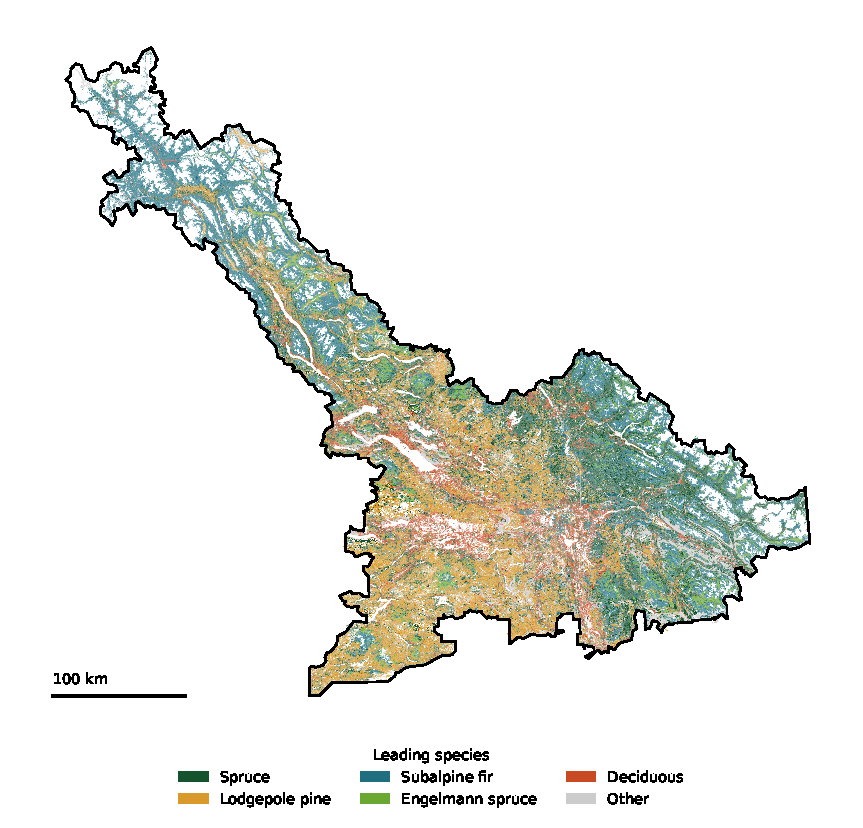
\includegraphics[width=0.75\linewidth]{figures/studyArea_map.pdf}
    \caption{The Prince George Timber Supply Area (TSA~24), showing the leading species of the
    stand inventory. Contains information licensed under the Open Government Licence -- British
    Columbia.}
    \label{fig:meth:modelregion}
\end{figure}

% Requires: \usepackage{booktabs}
\begin{table}[h]
    \centering
    \caption{Species composition of the managed land base (\SI{3.06}{\mega\hectare}) and of
    harvested volume in the reference schedule.}
    \label{tab:meth_studyregion_spec}
    \begin{tabular}{lrr}
        \toprule
        Species group & Area share [\%] & Harvested share [\%] \\
        \midrule
        Spruce (Sx)                        & 44.9 & 45.2 \\
        Lodgepole pine (Pl)                & 29.4 & 31.3 \\
        Subalpine fir (Bl)                 & 16.3 & 14.7 \\
        Trembling aspen (At)               & 5.3  & 5.3  \\
        Engelmann spruce (Se)              & 4.0  & 3.4  \\
        Black cottonwood (Ac)              & 0.1  & 0.1  \\
        \midrule
        Deciduous, all                    & 5.4  & 5.4  \\
        \bottomrule
    \end{tabular}
\end{table}

\subsection{Decision structure}

We analyse two layers of decision. A policy layer sets a harvest level and a post-clearcut stocking
standard; an enterprise layer responds with a harvest schedule. The standard specifies the species
composition of a plantation, and the landscape composition is an outcome.

This is a policy evaluation, not a bilevel program: the standard is exogenous and no equilibrium is
claimed. We hold the enterprise's harvest schedule at the even-flow plan and vary the standard, so
the comparison isolates the effect of what is planted at a fixed harvest pattern. A full enterprise
response---changing which blocks are harvested and how much---is outside the scope of this paper.

\paragraph{Enterprise level} The even-flow schedule is the enterprise's baseline plan. It was
produced by a weighted goal program that minimises weighted deviations from the harvest level and
even-flow aspirations, subject to area balance and the treatment options on each block
\citep{ubc_fresh_ws4_2026}. The minimum and maximum are one-sided penalty terms, not feasibility
bounds, so the realised cut is an outcome of the weighted compromise. We keep that schedule for
every standard. The species regenerated on each block are set by the standard.

\paragraph{Policy levels and standards} The harvest levels are \SI{100}{\percent},
\SI{80}{\percent}, and \SI{60}{\percent} of the even-flow plan, implemented as a deterministic block
sample that keeps each block's full harvest history. The standards are the historical clearcut
(\texttt{CC}) and three deciduous-forward prescriptions: \texttt{CC\_D26}, \texttt{CC\_D55}, and
\texttt{CC\_D84}, targeting 26, 55, and 84 percent deciduous. A standard is applied only where it
increases the deciduous share of the source analysis unit; aspen blocks stay on \texttt{CC}. The
realised composition is reported beside every policy.

\paragraph{Scope of the risk analysis} We report a policy ranking conditional on the recorded fire
regime, not a fire-size prediction. The standard changes the severity of a fire that reaches a
stand, not the number or size of fires. Each draw uses one event set for every policy, so the
comparison is paired. The no-fire net present value is the counterfactual; the fire loss is the
difference. CVaR20 is the mean loss in the worst 20 percent of draws, and the difference is reported
with a paired bootstrap interval.

\subsection{Forest estate model and estate data}

The model is implemented in \textsc{ws4}, the spatially explicit estate model of the UBC FRESH
laboratory \citep{ubc_fresh_ws4_2026}. The baseline compiled dataset contains \num{458708} blocks
and 48 treatments; the policy dataset adds the three prescriptions. Growth, treatment, and
transition information are carried as curves per block, compiled from the provincial inventory and
the timber supply analysis. The management process sets the regenerated cohort species to the
target track's composition.

We run 20 periods of ten years. The even-flow search converges to a realised level of
\SI{51.89}{\mega\cubic\meter} to \SI{52.06}{\mega\cubic\meter} per period, a mean of
\SI{5.19}{\mega\cubic\meter\per\year}. We treat this as the estate's sustained even-flow level, not
a proven maximum. The level is below the official cut; \autoref{sec:results} attributes the gap to
the flow rule rather than treating the official cut as a model constraint. The policy surface
samples 100, 80, and 60 percent of the plan's blocks; the realised level is reported for each
policy.

\subsection{Growth and yield}

Growth is represented by species-resolved yield curves compiled per block from the TSA~24 inventory
bundle. The curves carry the site-specific volume, height, and species trajectories on which the
harvest and regeneration decisions act. They are fixed trajectories and do not respond to climate,
changing site productivity, or within-stand species interactions; the discussion returns to this.

\subsection{Fire regime and composition-dependent severity}

The fire regime is the full TSA~24 record: \num{1073} perimeters from 1950 to 2024,
\num{14.31} fires per year, \SI{10079}{\hectare\per\year}, a mean fire of \SI{704.5}{\hectare},
and a maximum of \SI{72317}{\hectare}. The record is a mapped-fire history, not a forecast: small
fires are under-recorded, the record spans changing suppression and climate, and the tail rests on
a small number of events.

The policy surface uses the recorded size and frequency distribution with a composition-dependent
severity model, which holds the regime fixed and isolates the fuel effect. The calibrated
surface-fire model \citep{ubc_fresh_fire_calibration_2026} validates the regime and demonstrates
estate coupling; its per-tile suppression parameters were fitted on 24 tiles against 432 historical
perimeters. The fit places the median and the share above \SI{500}{\hectare} inside the historical
sampling interval and the 95th percentile below it. A 24-ignition estate run shows that the
calibrated model couples to the harvest model.

\paragraph{Fuel projection} The 2025 VRI fuel type is the baseline for every unharvested stand. For
a harvested stand we follow the BC fuel-typing chronology: slash (S1) for 0--5 years, open
herb/grass (O1B) for 6--24 years, and the species-based forest type from year 25. The forest type
uses the calibrated VRI-to-FBP mapping, with the 30 percent mixedwood threshold used in the fire
calibration; the BC 2017 algorithm's 20 percent threshold is a sensitivity. The baseline is not
re-typed: re-typing every stand from the compiled analysis-unit composition reproduces 63.1 percent
of the operational grid, because the compiled dataset carries one species mix per analysis unit
while the VRI grid carries one per polygon. The mapping is consistent with the operational layer on
real stands: 529 aspen-dominated polygons aged 25 or more are D1, 171 polygons at 40--60 percent
deciduous are M1 or M2, and 357 polygons at 20--30 percent deciduous are conifer types.

\paragraph{Severity} A fire that reaches a stand kills a fraction of its biomass. We compute the
FBP crown fraction burned (CFB) for the stand's fuel type under the calibration weather
(FFMC~93.8, BUI~108.2, wind~\SI{6.8}{\kilo\meter\per\hour}) and map it onto the process severity
bounds:
\[
  \text{raw severity} = 0.2 + 0.8\,\text{CFB}.
\]
We normalise by the initial-landscape area-weighted mean (0.7496), so a multiplier of one is the
calibrated landscape mean. The multiplier scales the burned-area mortality fraction in the fire
process. The gradient is non-linear: under the calibrated 30 percent threshold, the 26 percent
standard stays on the conifer side (C2/C1, multiplier 1.299 or 0.749), the 55 percent standard is
M1 (1.011), and only the 84 percent standard is D1 (0.267). Under the BC 20 percent threshold, the
26 percent standard becomes M2 (1.203), still only 7 percent below closed spruce.

\paragraph{Design} Ten draws of the full record over 200 years. Each draw generates one event set
and applies it to every policy, so the comparison is paired. The no-fire net present value is the
counterfactual; the fire loss is the difference. CVaR20 is the mean loss in the worst 20 percent of
draws, and the difference is reported with a paired bootstrap interval.

\subsection{Economic valuation}

Harvested volume is valued by species group at BC interior log prices for the three months ending
30 September 2026: \SI{113.96}{CAD\per\cubic\meter} for spruce and pine,
\SI{105.98}{CAD\per\cubic\meter} for subalpine fir on the hemlock--balsam series, which is the
nearest reported grade for that species, and a range of
\SIrange{35}{40}{CAD\per\cubic\meter} for deciduous species. Costs are a tree-length ground harvest system at
\SI{21.38}{CAD\per\cubic\meter} from machine rates, haul at \SI{7.85}{CAD\per\cubic\meter} over a
mean distance of \SI{90}{\kilo\meter} to the nearest sawmill, basic silviculture at
\SI{10.02}{CAD\per\cubic\meter} for the North Central zone, and stumpage at
\SI{9.92}{CAD\per\cubic\meter} for conifers and \SI{0.50}{CAD\per\cubic\meter} for deciduous
timber in grades 1 and 2. Net present value is computed at a \SI{3}{\percent} real discount rate, with each period's
net value discounted at its end. The net present value is an operating margin: it excludes road
construction, administration, taxes, and risk premia.

\subsection{Sensitivity and reproduction}

Three economic constants are ranges rather than points: the deciduous price, the haul distance, and
the discount rate. Every economic result is reported with a sensitivity across those ranges. The
severity model uses the calibration weather; the sensitivity of the multipliers to wind and the
surface-mortality floor is reported in the online supplement. All constants, their sources, and the
code that applies them are documented in the archived analysis repository.
